\documentclass[12pt, twoside]{article}
\usepackage[utf8]{inputenc}
\usepackage[english]{babel}

\usepackage{graphicx, subfigure, wrapfig, float}
\usepackage{amsmath, amssymb, amsfonts, amsthm}
\usepackage{caption, multicol, multirow, longtable}
\usepackage{url, cclicenses, lastpage, color, booktabs}
\usepackage{graphicx,lipsum,wrapfig} 
\usepackage{hyperref}
\usepackage{fancyhdr, fancybox}
\usepackage{array} 
\usepackage{vmargin}
\usepackage{xcolor}
\usepackage{listings}
\usepackage{url}

\def\blankpage{%
      \clearpage%
      \thispagestyle{empty}%
      \addtocounter{page}{-1}%
      \null%
      \clearpage}
      
\let\oldlstlistoflistings\lstlistoflistings
\renewcommand{\lstlistoflistings}{%
  \begingroup%
  \let\oldnumberline\numberline%
  \renewcommand{\numberline}{\lstlistingname~\oldnumberline}%
  \oldlstlistoflistings%
  \endgroup}


\usepackage{fancyvrb}

\RecustomVerbatimCommand{\VerbatimInput}{VerbatimInput}%
{fontsize=\footnotesize,
 %
 frame=lines,  % top and bottom rule only
 framesep=.3em, % separation between frame and text
 %
 labelposition=topline,
 %
 commandchars=\|\(\), % escape character and argument delimiters for
                      % commands within the verbatim
 commentchar=*        % comment character
}



%%%%%% Begin python listling

\usepackage{xcolor}
\definecolor{maroon}{cmyk}{0, 0.87, 0.68, 0.32}
\definecolor{halfgray}{gray}{0.55}
\definecolor{ipython_frame}{RGB}{207, 207, 207}
\definecolor{ipython_bg}{RGB}{247, 247, 247}
\definecolor{ipython_red}{RGB}{186, 33, 33}
\definecolor{ipython_green}{RGB}{0, 128, 0}
\definecolor{ipython_cyan}{RGB}{64, 128, 128}
\definecolor{ipython_purple}{RGB}{170, 34, 255}


\lstset{
    breaklines=true,
    %
    extendedchars=true,
    literate=
    {á}{{\'a}}1 {é}{{\'e}}1 {í}{{\'i}}1 {ó}{{\'o}}1 {ú}{{\'u}}1
    {Á}{{\'A}}1 {É}{{\'E}}1 {Í}{{\'I}}1 {Ó}{{\'O}}1 {Ú}{{\'U}}1
    {à}{{\`a}}1 {è}{{\`e}}1 {ì}{{\`i}}1 {ò}{{\`o}}1 {ù}{{\`u}}1
    {À}{{\`A}}1 {È}{{\'E}}1 {Ì}{{\`I}}1 {Ò}{{\`O}}1 {Ù}{{\`U}}1
    {ä}{{\"a}}1 {ë}{{\"e}}1 {ï}{{\"i}}1 {ö}{{\"o}}1 {ü}{{\"u}}1
    {Ä}{{\"A}}1 {Ë}{{\"E}}1 {Ï}{{\"I}}1 {Ö}{{\"O}}1 {Ü}{{\"U}}1
    {â}{{\^a}}1 {ê}{{\^e}}1 {î}{{\^i}}1 {ô}{{\^o}}1 {û}{{\^u}}1
    {Â}{{\^A}}1 {Ê}{{\^E}}1 {Î}{{\^I}}1 {Ô}{{\^O}}1 {Û}{{\^U}}1
    {œ}{{\oe}}1 {Œ}{{\OE}}1 {æ}{{\ae}}1 {Æ}{{\AE}}1 {ß}{{\ss}}1
    {ç}{{\c c}}1 {Ç}{{\c C}}1 {ø}{{\o}}1 {å}{{\r a}}1 {Å}{{\r A}}1
    {€}{{\EUR}}1 {£}{{\pounds}}1,
    tabsize=2
}

%%
%% Python definition (c) 1998 Michael Weber
%% Additional definitions (2013) Alexis Dimitriadis
%% modified by me (should not have empty lines)
%%
\lstdefinelanguage{iPython}{
    morekeywords={access,and,break,class,continue,def,del,elif,else,except,exec,finally,for,from,global,if,import,in,is,lambda,not,or,pass,print,raise,return,try,while},%
    %
    % Built-ins
    morekeywords=[2]{abs,all,any,basestring,bin,bool,bytearray,callable,chr,classmethod,cmp,compile,complex,delattr,dict,dir,divmod,enumerate,eval,execfile,file,filter,float,format,frozenset,getattr,globals,hasattr,hash,help,hex,id,input,int,isinstance,issubclass,iter,len,list,locals,long,map,max,memoryview,min,next,object,oct,open,ord,pow,property,range,raw_input,reduce,reload,repr,reversed,round,set,setattr,slice,sorted,staticmethod,str,sum,super,tuple,type,unichr,unicode,vars,xrange,zip,apply,buffer,coerce,intern},%
    %
    sensitive=true,%
    morecomment=[l]\#,%
    morestring=[b]',%
    morestring=[b]",%
    %
    morestring=[s]{'''}{'''},% used for documentation text (mulitiline strings)
    morestring=[s]{"""}{"""},% added by Philipp Matthias Hahn
    %
    morestring=[s]{r'}{'},% `raw' strings
    morestring=[s]{r"}{"},%
    morestring=[s]{r'''}{'''},%
    morestring=[s]{r"""}{"""},%
    morestring=[s]{u'}{'},% unicode strings
    morestring=[s]{u"}{"}
    %
    % {replace}{replacement}{lenght of replace}
    % *{-}{-}{1} will not replace in comments and so on
    literate=
    {á}{{\'a}}1 {é}{{\'e}}1 {í}{{\'i}}1 {ó}{{\'o}}1 {ú}{{\'u}}1
    {Á}{{\'A}}1 {É}{{\'E}}1 {Í}{{\'I}}1 {Ó}{{\'O}}1 {Ú}{{\'U}}1
    {à}{{\`a}}1 {è}{{\`e}}1 {ì}{{\`i}}1 {ò}{{\`o}}1 {ù}{{\`u}}1
    {À}{{\`A}}1 {È}{{\'E}}1 {Ì}{{\`I}}1 {Ò}{{\`O}}1 {Ù}{{\`U}}1
    {ä}{{\"a}}1 {ë}{{\"e}}1 {ï}{{\"i}}1 {ö}{{\"o}}1 {ü}{{\"u}}1
    {Ä}{{\"A}}1 {Ë}{{\"E}}1 {Ï}{{\"I}}1 {Ö}{{\"O}}1 {Ü}{{\"U}}1
    {â}{{\^a}}1 {ê}{{\^e}}1 {î}{{\^i}}1 {ô}{{\^o}}1 {û}{{\^u}}1
    {Â}{{\^A}}1 {Ê}{{\^E}}1 {Î}{{\^I}}1 {Ô}{{\^O}}1 {Û}{{\^U}}1
    {œ}{{\oe}}1 {Œ}{{\OE}}1 {æ}{{\ae}}1 {Æ}{{\AE}}1 {ß}{{\ss}}1
    {ç}{{\c c}}1 {Ç}{{\c C}}1 {ø}{{\o}}1 {å}{{\r a}}1 {Å}{{\r A}}1
    {€}{{\EUR}}1 {£}{{\pounds}}1
    %
    {^}{{{\color{ipython_purple}\^{}}}}1
    {=}{{{\color{ipython_purple}=}}}1
    %
    {+}{{{\color{ipython_purple}+}}}1
    *{-}{{{\color{ipython_purple}-}}}1
    {*}{{{\color{ipython_purple}$^\ast$}}}1
    {/}{{{\color{ipython_purple}/}}}1
    %
    {+=}{{{+=}}}1
    {-=}{{{-=}}}1
    {*=}{{{$^\ast$=}}}1
    {/=}{{{/=}}}1,
    %
    identifierstyle=\color{black}\ttfamily,
    commentstyle=\color{ipython_cyan}\ttfamily,
    stringstyle=\color{ipython_red}\ttfamily,
    keepspaces=true,
    showspaces=false,
    showstringspaces=false,
    %
    rulecolor=\color{ipython_frame},
    frame=single,
    frameround={t}{t}{t}{t},
    framexleftmargin=6mm,
    xleftmargin=.28in,
    numbers=left,
    numberstyle=\tiny\color{halfgray},
    %
    %
    backgroundcolor=\color{ipython_bg},
    %   extendedchars=true,
    basicstyle=\scriptsize,
    keywordstyle=\color{ipython_green}\ttfamily,
}
%%%%%% End python listling



%%%% My usual import
\usepackage{amsmath, amsthm, amssymb, calrsfs, wasysym, verbatim, bbm, color, graphics,  enumitem, listings, tcolorbox, tikz, newtxmath, pgfplots, hyperref, paracol}

\definecolor{td}{RGB}{170,0,0}

\renewcommand\rmdefault{lmr}


%%% My commands
\newcommand\projectTitle{Computer Scientists Retrieval}
\newcommand\school{Engineering in Computer Science}


\pagestyle{fancy}
\fancyhf{}

\fancyhead[LE]{\school}
\fancyhead[RE]{\projectTitle}



\fancyhead[RO]{Academic Year 2019-2020} \fancyhead[LO]{\school}
\cfoot{\thepage}

\begin{document}
\begin{titlepage}

\setmargins{2.5cm}{1cm}{16.5cm}{23.42cm}{10pt}{1cm}{0pt}{1cm}

%encabezado portada
\begin{figure}[t]
\begin{minipage}{0.5\textwidth}\large
\begin{flushleft}
%%%%	INSERIMENTO IMMAGINE IN ALTO A SINISTRA

%
\includegraphics[scale=0.15]{ECI.png}
\end{flushleft}
\end{minipage}
\begin{minipage}{0.5\textwidth}\large
\begin{flushright}

%%%%	INSERIMENTO IMMAGINE IN ALTO A DESTRA


\includegraphics[scale=.6]{images/ECI.png}
\end{flushright}
\end{minipage}
\end{figure}

%~~~~~~~~~~~~MODIFICAR~~~~~~~~~~~~~~~~~~~~~
\title{\textsc{Computer Scientists Retrieval}} 
%~~~~~~~~~~~~~~~~~~~~~~~~~~~~~~~~~~~~~~~~~~~~
\date{}
\maketitle

\vspace{16pt}

\noindent\begin{tabular}{p{6cm} p{10cm}}
\textcolor{td}{\rule{4.5cm}{0.04cm}} 
\par\medskip
\textbf{WIR Project}
\par\bigskip
\textbf{Students:}
\begin{itemize}
%~~~~~~~~~~~~~~~~TEAM~~~~~~~~~~~~~~~~~~~~~~
\item Luca Tomei
\item Daniele Iacomini
\item Andrea Aurizi
%~~~~~~~~~~~~~~~~~~~~~~~~~~~~~~~~~~~~~~~~~~~~~~~
\end{itemize}
\par\medskip
\textbf{Directed by:}
\par\bigskip


%\par\medskip \hspace{0.5cm}
%~~~~~~~~~~~~~~~~PROFS~~~~~~~~~~~~~~~~~~~~~~
\textrm{\textit{Andrea Vitaletti}}
\par\medskip
\textrm{\textit{Luca Becchetti}}

\vspace{15pt}
\href{https://github.com/LucaTomei/Computer_Scrientists}{\textit{\underline{Project Repository}}}

%~~~~~~~~~~~~~~~~~~~~~~~~~~~~~~~~~~~~~~~~~~~~~~~
\vspace{2cm} 
\par\medskip
\begin{center}
%~~~~~~~~~~~~~~~~AY~~~~~~~~~~~~~~~~~~~~~~
\textbf{A.Y. 2019-2020}
%~~~~~~~~~~~~~~~~~~~~~~~~~~~~~~~~~~~~~~~~~~~~~~~~
\end{center}
%~~~~~~~~~~~~~~~~~~~~~~~



%~~~~~~~~~~~~~~~~~~~~~~~~~~~~~~~~~~~~~~~~~~~~~~~~~~~~~~~~

\includegraphics[scale=0.4]{images/logo.png}
&

\textbf{Summary}	%Write Summary
\par\medskip
The paper we chose presents a method to find the most influential rock guitarist by applying Google’s PageRank algorithm to information extracted from Wikipedia articles. The influence of a guitarist is computed by considering the number of guitarists citing him/her as influence.
\linebreak

Basically, the experiment consists of building a directed graph where nodes are rock guitarists. There is an outgoing edge from guitarist A to another guitarist B, if guitarist A is influenced by guitarist B.
\begin{center}
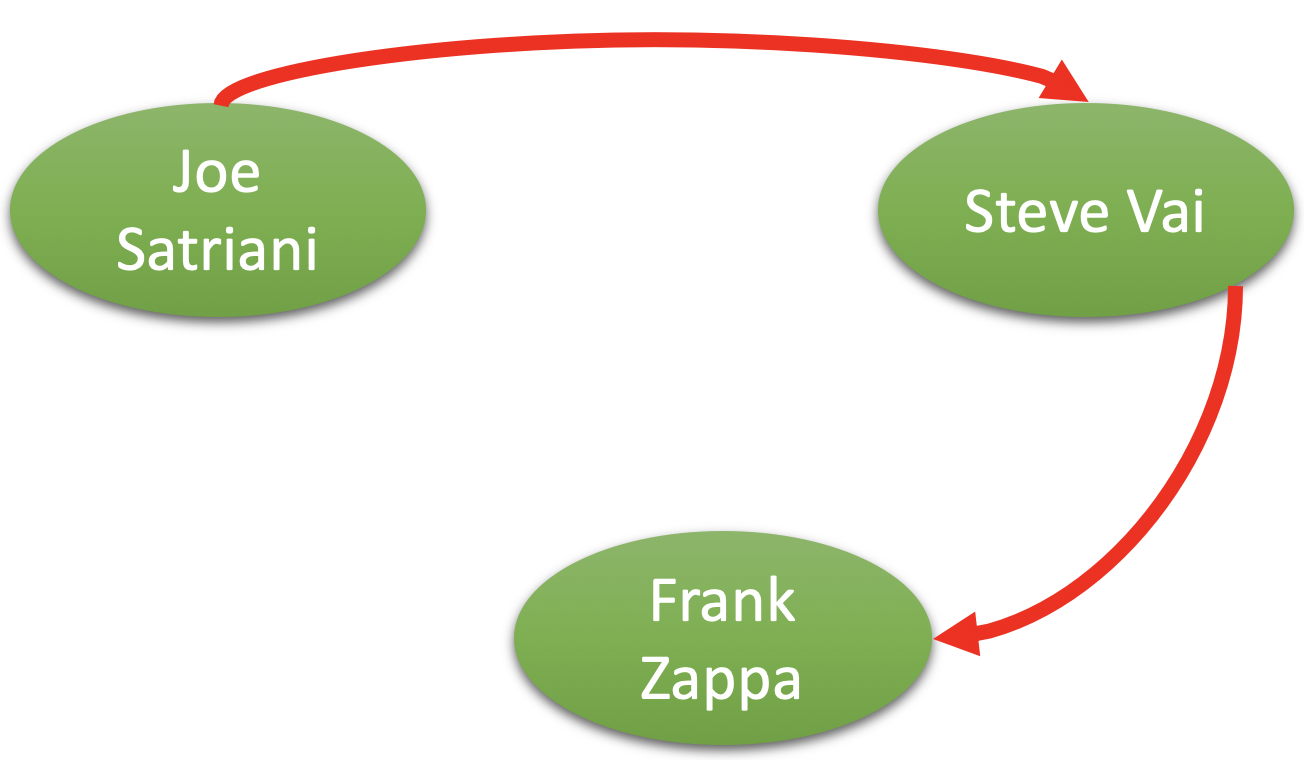
\includegraphics[scale=0.22]{images/guitar_influences}	
\linebreak
\scriptsize Joe Satriani is influenced by Steve Vai and the latter by Frank Zappa
\end{center}
We decided to replicate the same experiment with the same methodology but choosing computer scientists as the field of study.

\end{tabular}
\end{titlepage}

\tableofcontents
$\ $

\newpage
%%%%%%%%%%%%%%%%%%%%%%%%INTRODUCTION%%%%%%%%%%%%%%%%%%%%%%%%
\section{Introduction}
%In questo progetto ci siamo soffermati sull'analisi dei dati riguardanti una categoria diversa da quella dei chitarristi: i computer scientists. A differenza di un chitarrista o di un filosofo, un ingegnere informatico non ha molti dati rilevanti su wikipedia e non vi sono nemmeno informazioni riguardanti la sua scuola di pensiero o le influenze avute durante la sua vita. Infatti la prima difficoltà riscontrata durante la fase preliminare del progetto è stata proprio quella di cercare di creare una corrispondenza biunivoca tra due ingegneri informatici, cosa che non sempre è possibile.
In this project we focused on the analysis of data concerning a different category from that of guitarists: computer scientists. Unlike a guitarist or a philosopher, a computer engineer does not have much relevant data on wikipedia and there is also no information regarding his school of thought or the influences he had during his life. In fact, the first difficulty encountered during the preliminary phase of the project was precisely to try to create a one-to-one correspondence between two computer scientists, which is not always possible.

\begin{figure*}[htp]
\begin{minipage}[t]{0.5\linewidth}
\centering
	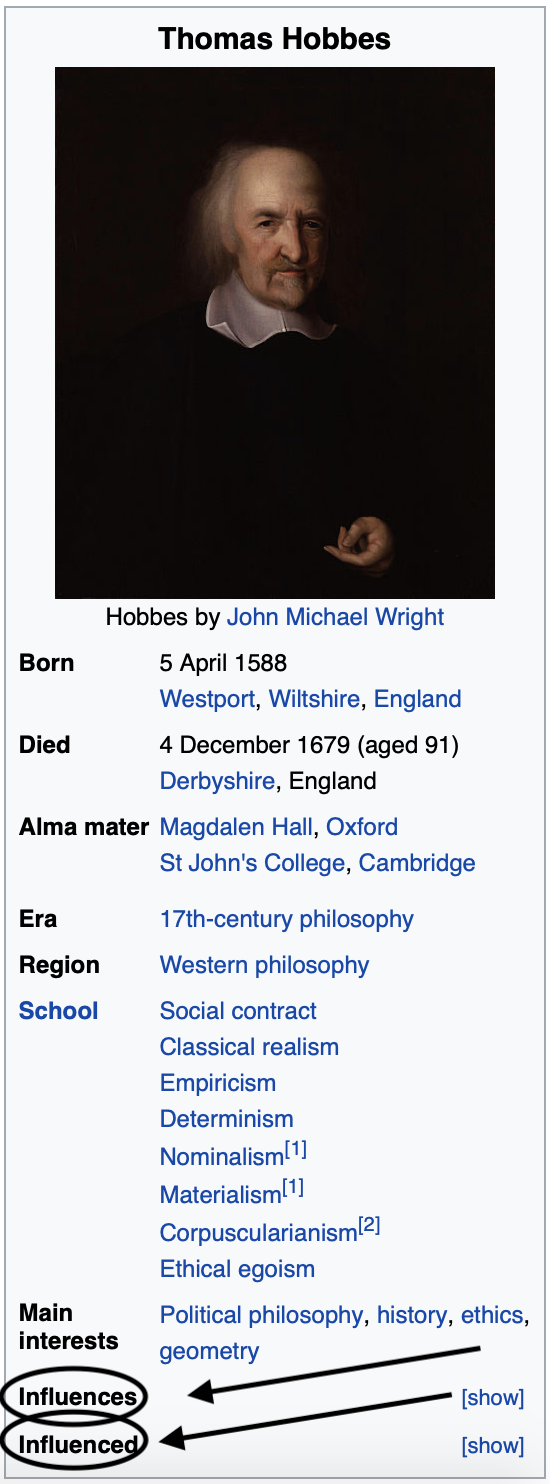
\includegraphics[width = .5\textwidth]{images/hobbes}
\end{minipage}
\begin{minipage}[t]{0.5\linewidth}
\vspace{-260pt}
\centering

\includegraphics[width = .5\textwidth]{images/van_der}
\end{minipage}
\caption{Poet vs Computer Scientist}
\end{figure*}
\noindent
%Le precedenti figure mostrano i campi dati presenti sulle tabelle "infobox biography vcard" di WikiPedia. La differenza nel numero di campi tra un filosofo ed un computer scientist è netta ed inoltre quest'ultimo non presenta campi di tipo "Influences" e "Influenced" a cui possiamo attingere per creare collegamenti tra un informatico ed un altro.\\
The previous figures show the data fields on the WikiPedia "infobox biography vcard" tables. The difference in the number of fields between a philosopher and a computer scientist is clear and the latter also has no "Influences" and "Influenced" type fields that we can draw on to create connections between one computer scientist and another. \\
%Pertanto, per ovviare a tale problema, in primo luogo si è deciso di utilizzare \textit{SPARQL} per esplorare ed estrarre le informazioni contenute in grafi RDF da una base di conoscenza distribuita su \textit{DBpedia}.\\
Therefore, to overcome this problem, we first decided to use \textit{SPARQL} to explore and extract the information contained in RDF graphs from a knowledge base distributed on \textit{DBpedia}.\\
%Successivamente si è deciso di effettuare una ulteriore verifica dei risultati andando ad interrogare direttamente Wikipedia dato che è senza dubbio una delle maggiori risorse del Web per tutte le conoscenze.
Subsequently it was decided to carry out a further verification of the results by going directly to Wikipedia since it is undoubtedly one of the greatest resources of the Web for all knowledge.
\newpage
\section{Query DBpedia with SPARQL}
%Per interrogare DBpedia si è pensato di utilizzare \textit{SPARQLWrapper}, wrapper con lo scopo di a creare l'URI della query e, possibilmente, a convertire il risultato in un formato più gestibile.
To query DBpedia it was decided to use \textit{SPARQLWrapper}, wrapper with the aim of creating the URI of the query and possibly converting the result into a more manageable format.
\vspace{6pt}
\begin{lstlisting}[caption={Query DBpedia},captionpos=b,language=iPython]
"""Query DBpedia with SPARQL Code"""
from SPARQLWrapper import SPARQLWrapper, JSON

def query_dbpedia(self):
    sparql = SPARQLWrapper("http://dbpedia.org/sparql")
    sparql.setQuery("""
        PREFIX dbo: <http://dbpedia.org/ontology/>
        PREFIX foaf: <http://xmlns.com/foaf/0.1/>
        PREFIX dct: <http://purl.org/dc/terms/>
        PREFIX dbr: <http://dbpedia.org/resource/>
        PREFIX dbc: <http://dbpedia.org/resource/Category:>

        SELECT distinct ?name  ?person ?subject WHERE {
          ?person foaf:name ?name. 
          ?person dct:subject dbc:Computer_scientists.  
          ?person dct:subject ?subject.
        filter regex(?subject, "http://dbpedia.org/resource/Category:Computer_scientists")
        }
        ORDER BY ?name
    """)
    sparql.setReturnFormat(JSON)
    results = sparql.query().convert()
    return results
\end{lstlisting}
%Dopo aver incapsulato l'output della query nella variabile \lstinline[language = iPython]{result} siamo pronti ad esaminare i dati ottenuti e a creare un grafo per calcolare il pagerank.
After encapsulating the query output in the variable \lstinline[language = iPython]{result} we are ready to examine the data obtained.\\
Going to analyze the updated data, we realized that in many cases the same person is registered in multiple repositories but under different URIs. However, only a small part of the possible links between them is available.\\
Since there is no ontology regarding computer scientists, more links can be discovered by performing automatic coreference resolution, but this task is complicated by two issues:
\begin{itemize}[noitemsep, topsep=0pt]
	\item Datasets do not contain overlapping properties for their individuals apart from personal names.
	\item 	Individuals which belong to overlapping subsets are not distinguished from others: in DBPedia the majority of computer scientists is assigned to a generic class \textit{dbpedia:Person} and not distinguished from other people. As a result, it becomes complicated to extract the subset of computer scientists from DBPedia.
\end{itemize}
Individuals in DBPedia are connected by \textit{rdf:type} links to classes defined in the YAGO repository. The YAGO ontology is based on Wikipedia categories and provides a more detailed hierarchy of classes than the DBPedia ontology.\\
The data returned by the query are not satisfactory, therefore it was decided to take a winding road: the manual scraping of wikipedia pages.





\newpage

\section{Manual scraping Wikipedia}
%DBpedia offre pochi risultati per i Computer Scientists, motivo per cui si è deciso di intraprendere una strada più impegnativa ma che ci restituisse più risultati: il Web Scarping.\\
DBpedia offers few results for Computer Scientists, which is why it was decided to take a more demanding path but that would give us more results: Web Scarping. \\
%Si è pensato di suddividere tale processo in 4 fasi logiche:
%\begin{enumerate}[noitemsep, topsep=1pt]
%	\item Collezionare in un file tutti i link di computer scientists presenti nella versione inglese di Wikipedia (\textit{\href{https://en.wikipedia.org/wiki/List_of_computer_scientists}{List Of Computer Scientists}}).
%	\item Per ogni link di un informatico ottenuto dalla fase precedente, si è verificato se la relativa pagina web contenesse una tabella informazioni che includesse la lista di influenze e influenzati di tale informatico. 
%	\item Dai risultati ottenuti si è calcolato il Pagerank con lo scopo di quantificare l'importanza dell'informatico relativa all'interno dell'insieme di documenti connessi.
%	\item Si è pensato di soffermarci sulla classificazione dei vari campi di studio di un informatico.
%\end{enumerate}
It was decided to divide this process into 4 logical phases:
\begin{enumerate}[noitemsep, topsep=1pt]
	\item Collect in a file all the links of computer scientists present in the English version of Wikipedia (\textit{\href{https://en.wikipedia.org/wiki/List_of_computer_scientists}{List Of Computer Scientists}}).
	\item For each link of a computer scientist obtained from the previous phase, it was checked whether the relative web page contained an information table that included the list of influences and influences of this computer scientist.
	\item From the results obtained, the Pagerank was calculated with the aim of quantifying the importance of the relative computer scientist within the set of related documents.
	\item It was decided to dwell on the classification of the various fields of study of a computer scientist.
\end{enumerate}

\subsection{First Phase: Collect data}
The English version of Wikipedia contains a list of all the computer scientists (\textit{\href{https://en.wikipedia.org/wiki/List_of_computer_scientists}{link}}) with an existing article, alphabetically sorted. In the first phase, we simply copy each link and its associated name in a .json file.\\
The total number of computer scientists retrieved is 509.

\subsection{Second Phase: Check informations in  Biographic Table}
%Prima di iniziare ad estrapolare le informazioni di ogni informatico, per un questione di ottimizzazione del codice e di efficienza in termini prestazionali si è pensato di rendere offline le intere pagine Wikipedia di ognuno di essi, in modo tale da non effettuare $n\_cs = 509$ richieste.\\
Before starting to extrapolate the information of each computer scientist, for a matter of code optimization and efficiency in terms of performance it was decided to download the entire Wikipedia pages of each of them, so as not to make $ n\_cs =  509$ requests. \\
%Dopo aver collezionato le pagine web di ogni informatico, per ognuno di essi si è verificato se la corrispettiva pagina contenesse una tabella informativa  (\textit{Infobox} HTML) che includesse la lista di influences and influencers del suddetto informatico.
After collecting the web pages of each computer scientist, for each of them it was checked whether the corresponding page contained an information table (\textit{Infobox} HTML) which included the list of influences and influencers of the said computer scientist.

%Il numero di Computer Scientists che soddisfano tale requisito è pari a $62$.
The number of Computer Scientists who meet this requirement is $ 62 $.
\begin{lstlisting}[language = iPython, caption={Checking Bio Table Function},captionpos=b]
def bio_table(self, page):
    name = page.rsplit('/')[-1]
    page = open(page, 'r')
    soup = BeautifulSoup(page, "html.parser")
    table = soup.find('table', class_='infobox biography vcard')
    try:	influencers = table.find_all('ul', class_='NavContent')[0]
    except:	influencers = []
    try:	influenced = table.find_all('ul', class_='NavContent')[1]
    except:	influenced = []
    final_influencers, final_influenced = ([] for i in range(2))
    if influencers != []:
        for a in influencers.find_all('a'):
        	final_influencers.append(a.get('title'))
    if influenced != []:
        for a in influenced.find_all('a'):
        	final_influenced.append(a.get('title'))
\end{lstlisting}

\newpage
\subsection{Third Phase: Second Approach and Pagerank}
%Dato che il risultato ottenuto dalla seconda fase è stato per nulla soddisfacente, si è deciso di utilizzare un secondo approccio: invece di verificare solamente la tabella biografia di un informatico si è analizzata l'intera pagina a lui associata.
Since the result obtained from the second phase was not at all satisfactory, it was decided to use a second approach: instead of checking only the biography table of a computer scientist, the entire page associated with him was analyzed.
\vspace{6pt}
\begin{lstlisting}[language = iPython, caption={Making Links},captionpos=b]
def make_links(self, path):
	# Define output dict
	inlinks = SortedDict() 
	outlinks = SortedDict()

	SetofNames = SortedSet()

	#reading all the folders from the path and creating a set of CS names
	for name in self.read_names(path):
		if name == "Guy_L._Steele,_Jr":	name = "Guy_L._Steele,_Jr."

		SetofNames.add(name)

		#creating an empty inlinks of names as sortedSet
		inlinks[name] = SortedSet()

	#reading their inlinks and outlinks
	for name in SetofNames:
		SetOfInLinks = SortedSet()
		fp = open(path + "/"+ name,'r',encoding = "utf-8")
		soup = BeautifulSoup(fp.read(),"html.parser")
		linksFound = []
		linksFound = soup.findAll('a', href=re.compile("/wiki/"))

		HTML = ""
		for link in linksFound:
			HTML = HTML + str(link)
			HTML = HTML + " and "

		#get All the outlinks by calling get_links
		outlinks[name] = self.get_links(SetofNames,HTML)

		if name in outlinks[name]:	outlinks[name].remove(name)

		for outlink in outlinks[name]:
			SetOfInLinks.add(name)
			inlinks[outlink].update(SetOfInLinks)
	return (inlinks,outlinks)
\end{lstlisting}
The previous function, after reading the html pages of each computer scientist as input, creates and returns two \textit{SortedDict}:
\begin{itemize}[noitemsep, topsep=0pt]
	\item \textit{inlinks}: maps from a name to a SortedSet of names that link to it.
	\item \textit{outlinks}: maps from a name to a SortedSet of names that it links to.
\end{itemize}
For example:
\begin{itemize}[noitemsep, topsep=0pt]
	\item \lstinline[language = iPython]{inlinks['Ada_Lovelace'] = SortedSet(['Charles_Babbage', 'David_Gelernter'], key=None, load=1000)}
	\item \lstinline[language = iPython]{outlinks['Ada_Lovelace'] = SortedSet(['Alan_Turing', 'Charles_Babbage'], key=None, load=1000)}
\end{itemize}
To obtain all the \textit{outlinks} we call \lstinline[language = iPython]{self.get_links(SetofNames,HTML)}, which return a SortedSet of computer scientist names that are linked from this html page. The return set is restricted to those people in the provided set of names. The returned list should contain no duplicates. This function take as input:
\begin{itemize}[noitemsep, topsep=0pt]
	\item	A SortedSet of computer scientist names, one per filename.
	\item	A string representing one html page.
\end{itemize}

\newpage

\begin{lstlisting}[language = iPython, caption={Get Links},captionpos=b]
def get_links(self, names, html):
	listofHrefs = []
	listofHrefTexts = []
	FinalSortedSet = SortedSet()
	splice_char = '/'

	for i in range(0,len(listofHrefs)):
		value = listofHrefs[i][6:]
		listofHrefTexts.append(value)

	listofHrefTexts = re.findall(r"href="([^"]*)", html)

	for i in listofHrefTexts:
		value = i[6:]
		listofHrefs.append(value)
	listofHrefs = list(set(listofHrefs))

	for href in listofHrefs:
		for name in names:
			if(name == "Guy_L._Steele,_Jr"):
				names.remove(name)
				names.add("Guy_L._Steele,_Jr.")
			if(href == name):	FinalSortedSet.add(name)

	return FinalSortedSet
\end{lstlisting}

\noindent With the results obtained by the function \textit{make\_links} we can calculate the pagerank by calling the function \lstinline[language = iPython]{compute_pagerank}.
\vspace{6pt}
\begin{lstlisting}[language = iPython, caption={Computing Pagerank},captionpos=b]
def compute_pagerank(self, urls, inlinks, outlinks, b=.85, iters=20):
	rw = defaultdict(lambda:0.0)
	pageRank = defaultdict(lambda:1.0)

	for outlink in outlinks:	rw[outlink]=len(outlinks[outlink])

	#initialize page ranks scores to 1
	for url in urls:	pageRank[url] = 1.0

	for i in range(iters):
		for url in urls:
			summ = 0.0
			for link in inlinks[url]:	summ += 1.0 * pageRank[link]/rw[link]
			pageRank[url] = (1/len(urls))* (1.0-b)+b*summ
	return SortedDict(dict(pageRank))
\end{lstlisting}
This function return a \textit{SortedDict} mapping each url to its final PageRank value (float) by using this formula:
\begin{equation*}
	R(u) = \Big(\frac{1}{N}\Big) (1-b) + b \cdot \sum_{w \in B_u} \frac{R(w)}{|F_w|}
\end{equation*}
where: \begin{itemize}[noitemsep, topsep=0pt]
 	\item $R(u)$ = Pagerank value of the page $ u $ we want to calculate;
 	\item $B(u)$ = A set of pages that contain at least one link to the $ u $ page. $ w $ represents each of these pages;
 	\item $R(w)$ = PageRank values of each page	 $w$;
 	\item $F_w$ = Total number of links contained on the page offering the link;
 	\item $b$ = Damping factor. It is generally assumed that it will be set around 0.85.
 \end{itemize}
 \newpage
 
 \subsubsection{My Pagerank Results}
 The following figure shows the terminal output after making the call to \textit{compute\_pagerank} with 20 iterations e 509 computer scientists.
 \begin{figure*}[htp]
 	\centering
 	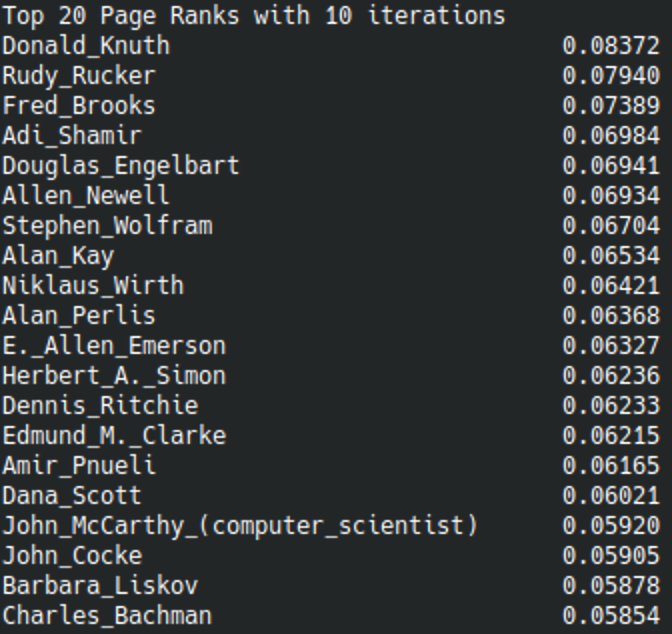
\includegraphics[width = .38\textwidth]{images/top_20_my_pagerank}
 	\caption{\textit{compute\_pagerank} output}
 \end{figure*}

\noindent
After applying the pagerank, it was decided to build a direct graph that highlighted the connections between each computer scientist. The figure shown below, built with the Python PIL library, shows that there is a thickening in the upper part which highlights the numerous connections that are among the top computer scientists obtained as an output from the \textit{compute\_pagerank} function.

\begin{figure*}[htp]
\centering
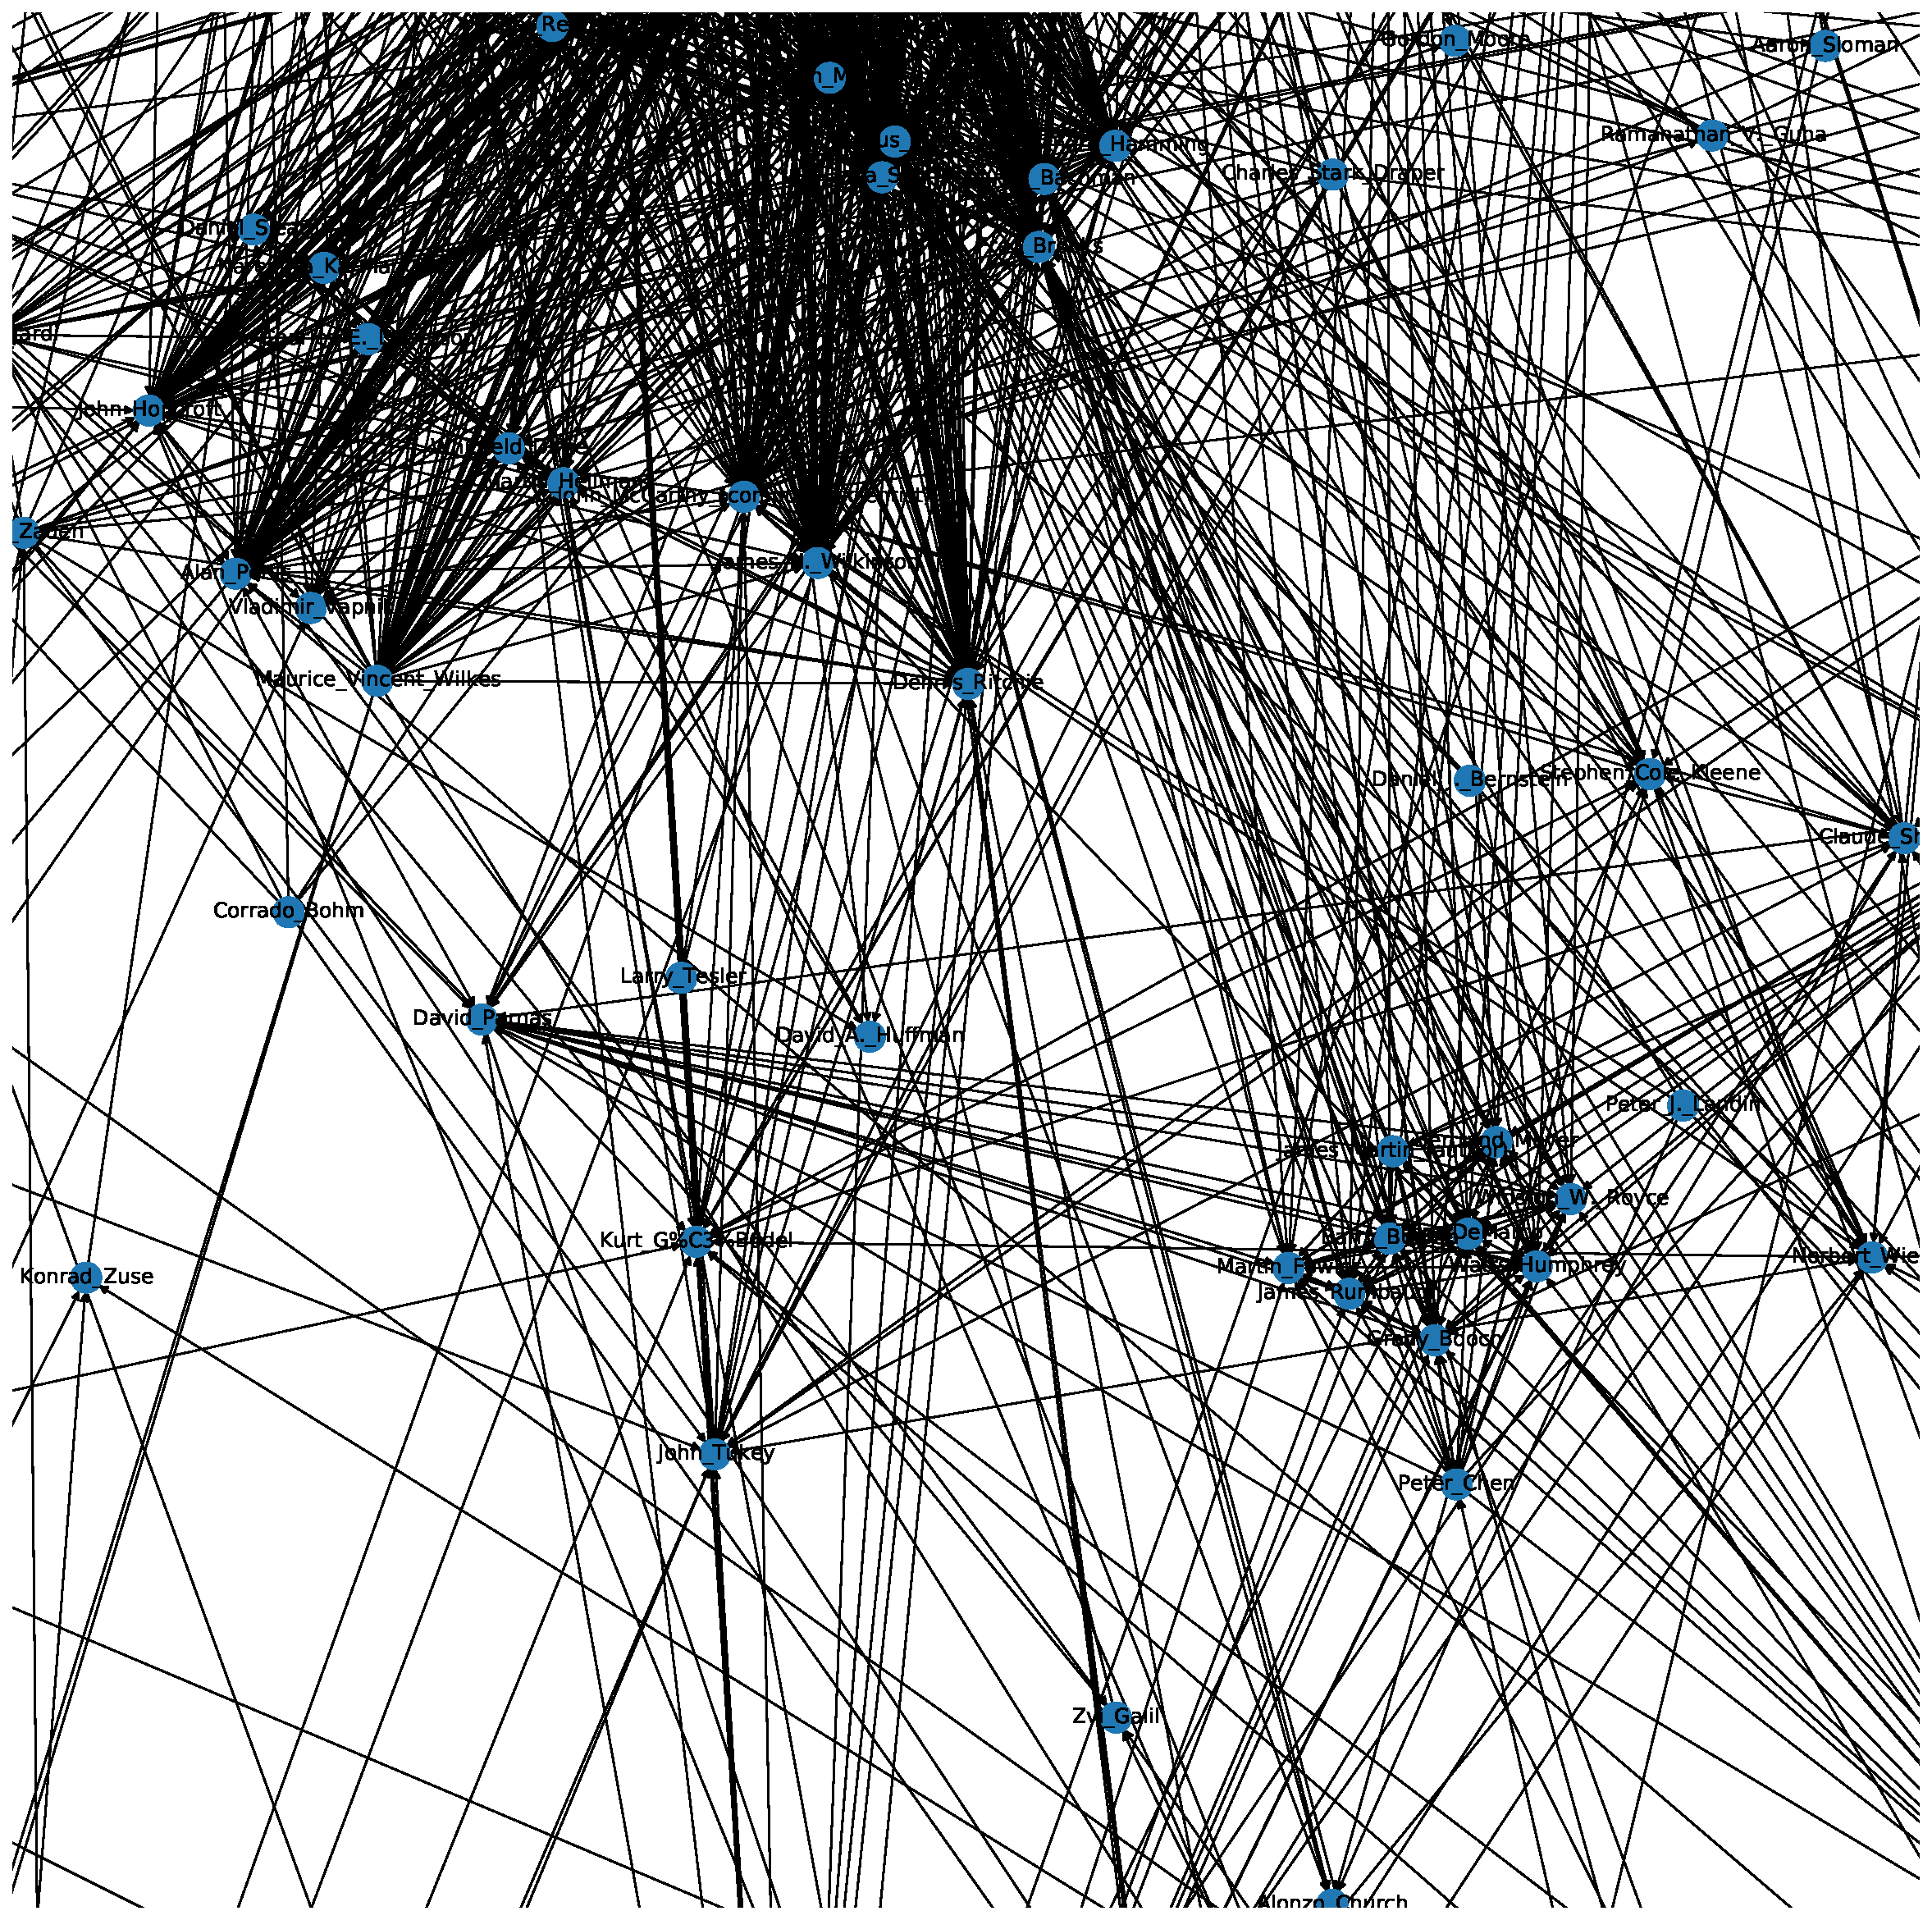
\includegraphics[width = .69\textwidth]{images/my_graph}
\caption{Pagerank Graph}
\end{figure*}

\newpage

\section{Categorization}
%Un'ulteriore esperimento è stato quello di cercare di stilare una classifica delle migliori branche di studio effettuate da tali persone.\\
A further experiment was to try to draw up a ranking of the best branches of study carried out by these people.\\
%Nella valutazione dei campi da poter utilizzare, si è verificato che la maggioranza dai computer scientist presenta nella famosa \textit{infobox table} di Wikipedia un campo di nome \textit{Field} che fa proprio al caso nostro: contiene ogni categoria di studio effettuata dalla persona che si sta esaminando.\\
In evaluating the fields that can be used, it has been verified that the majority of computer scientists present in the famous Wikipedia \textit{infobox table} a field called \textit{Field} which is right for us: it contains every category of study carried out from the person being examined.\\
%Su un totale di 509 computer scientist, tale campo è presente in circa 480 persone.\\
Out of a total of 509 computer scientists, this field is present in about 480 people. \\
%In basso a sinistra viene mostrato il codice utilizzato per estrapolare tale informazione ed in basso a destra una funzione atta a creare un file json che associa il nome di un computer scientist alle categorie di appartenenza.
In the lower left is shown the code used to extrapolate this information and a function designed to create a json file that associates the name of a computer scientist with the categories to which it belongs.

\noindent\begin{minipage}[t]{.52\linewidth}
\centering
\begin{lstlisting}[language = iPython, caption={Get Fields},captionpos=b]
def get_fields(self, file_name):
	soup = BeautifulSoup(self.get_html_content(file_name), 'html.parser')
	infobox = soup.find('table', {'class':'infobox'})
	fields_list = []
	if infobox != None:
		for item in infobox.findAll('tr'):
			infobox_key = item.find('th')
			if infobox_key != None and infobox_key.get_text() == 'Fields':
				infobox_value = item.find('td')
				fields_list.append(infobox_value.get_text())
	this_name = self.get_cs_name_from_filename(file_name)
	return fields_list
\end{lstlisting}

\end{minipage}\hfill
\noindent\begin{minipage}[t]{.46\textwidth}
\centering
\begin{lstlisting}[language = iPython, caption={Categorization },captionpos=b]
def compute_categorization(self, all_cs_files_list):
	to_ret = []
	none = 0
	for file_name in all_cs_files_list:
		cs_name = self.get_cs_name_from_filename(file_name)
		his_fields = self.clean_fields(self.get_fields(file_name))

		new_fields = []
		for item in his_fields:	new_fields.append(item.capitalize())
		if new_fields != []:
			cs_name = urllib.parse.unquote(cs_name)
			to_ret.append({cs_name:new_fields})
		else:
			none += 1
	return to_ret
\end{lstlisting}

\end{minipage}	
%\noindent Dopo aver ottenuto un file json contenente l'insieme ordinato di categorie associate ad un computer scientist, si è infine stilata una classifica attraverso la computazione dell'algoritmo pagerank e hits.\\
%Di seguito vengono mostrati i risultati ottenuti dai due algoritmi:
\noindent After obtaining a json file containing the ordered set of categories associated with a computer scientist, a ranking was finally drawn up through the computation of the pagerank and hits algorithm. \\
The results obtained by the two algorithms are shown below:

\begin{paracol}{2}
\VerbatimInput[fontsize=\tiny,label=$hits\_top\_20\_categories.txt$]{../../files/hits_top_20_categories.txt}
\switchcolumn
\VerbatimInput[fontsize=\tiny,label=$pagerank\_top\_20\_categories.txt$]{../../files/pagerank_top_20_categories.txt}
\end{paracol}



\newpage

\section{Conclusions}
The experiment consisted of applying the same procedure to computer scientists as described in the original document: the discrepancy between the rankings is minimal, especially if the list of the top twenty is taken into account (instead of just the list of the top ten). The complete rankings can be consulted on the Github page. One of the biggest difficulties in the experiment was polishing the data in order to provide reliable results. For this reason, the dataset obtained with DBpedia was not used in subsequent tests with custom HITS and PageRank. A larger number of datasets would have made the results of the experiment more interesting.
\section{Contacts}
Here is the GitHub link of our project: \href{https://github.com/LucaTomei/Computer_Scientists}{https://github.com/LucaTomei/Computer\_Scientists}


\newpage
\blankpage

\newpage
\listoffigures
\lstlistoflistings
\newpage

\begin{thebibliography}{X} %My Bibliography
\bibitem{SPARQLWrapper}	SPARQLWrapper: \href{https://pypi.org/project/SPARQLWrapper/}{https://pypi.org/project/SPARQLWrapper/}
\bibitem{bs4} bs4 Beautiful Soup: \href{https://www.crummy.com/software/BeautifulSoup/bs4/doc/}{https://www.crummy.com/software/BeautifulSoup/bs4/doc/}
\bibitem{urllib} urllib: \href{https://docs.python.org/3/library/urllib.html}{https://docs.python.org/3/library/urllib.html}
\bibitem{requests} requests: \href{https://requests.readthedocs.io/en/master/}{https://requests.readthedocs.io/en/master/}
\bibitem{re} Regular expression operations (re): \href{https://docs.python.org/3/library/re.html}{https://docs.python.org/3/library/re.html}
\bibitem{NetworkX} NetworkX: \href{https://networkx.github.io}{https://networkx.github.io}
\bibitem{Matplotlib} Matplotlib: \href{https://matplotlib.org/users/pyplot\_tutorial.html}{https://matplotlib.org/users/pyplot\_tutorial.html}
\bibitem{sortedcontainers} Sortedcontainers: \href{http://www.grantjenks.com/docs/sortedcontainers/}{http://www.grantjenks.com/docs/sortedcontainers/}
\bibitem{Collections} Collections: \href{https://docs.python.org/3/library/collections.html}{https://docs.python.org/3/library/collections.html}
\bibitem{Glog} Glob: \href{https://docs.python.org/2/library/glob.html}{https://docs.python.org/2/library/glob.html}
\bibitem{Tarfile} Tarfile: \href{https://docs.python.org/3/library/tarfile.html}{https://docs.python.org/3/library/tarfile.html}

\end{thebibliography}



\end{document}



